\documentclass[11pt, a4paper]{article}
\usepackage[utf8]{inputenc}
\usepackage[italian]{babel}
\usepackage{amsmath, amssymb}
\usepackage{geometry}
\usepackage{graphicx}
\usepackage{booktabs}
\usepackage{float}
\usepackage{hyperref}
\geometry{a4paper, margin=2.5cm}

\title{Checkpoint 2: Verso una Stima Quasi Perfetta\\
\large Copula Gaussiana Bivariata --- Attivazioni, Stabilità e Trasformazione degli Input}
\author{Edoardo Caproni, Pietro Pianigiani, Tommaso Quintabà\\
\small Corso di Statistical Machine Learning}
\date{3 Marzo 2026}

\begin{document}
\maketitle

% =========================================================================
\section{Motivazione}
% =========================================================================

Nel Checkpoint 1 abbiamo stabilito una pipeline funzionante e, attraverso un grid search, raggiunto una KL divergence di circa $0.010$ sulla copula gaussiana ($\rho = 0.7$). Tuttavia i plot 3D mostravano chiaramente che la rete (MLP con output \texttt{softplus}) faticava a catturare i picchi della copula agli angoli $(0,0)$ e $(1,1)$ del dominio $[0,1]^2$.

In questo checkpoint esploriamo sistematicamente tre direzioni per migliorare la stima:
\begin{enumerate}
    \item \textbf{Attivazione di output:} \texttt{softplus} vs.\ \texttt{exp} (Esperimento 3)
    \item \textbf{Gradient clipping:} stabilizzazione del training con \texttt{exp} (Esperimento 4)
    \item \textbf{Trasformazione degli input:} $\Phi^{-1}(u)$ come pre-processing (Esperimento 5)
\end{enumerate}

% =========================================================================
\section{Esperimento 3: Attivazione e scaling dei dati}
% =========================================================================

\subsection{Motivazione}

L'output \texttt{softplus}$(z) \approx z$ per $z \gg 0$ cresce linearmente: non può raggiungere valori arbitrariamente grandi senza logit enormi. La copula gaussiana con $\rho = 0.7$ raggiunge $c(u,v) \approx 13$ agli angoli della griglia di valutazione ($\varepsilon = 0.01$), dove \texttt{softplus} fatica.

L'attivazione \texttt{exp}$(z) = e^z$ cresce esponenzialmente e può raggiungere qualsiasi valore positivo. Inoltre semplifica il calcolo della NLL: $-\log(\exp(z)) = -z$, eliminando il passaggio per il logaritmo.

Testiamo anche l'effetto di aumentare $N$ (da 2000 a 10000) e di usare un cosine annealing scheduler per il learning rate.

\subsection{Setup}

Rete fissa: $128 \times 3$ (best da grid search), $\lambda = 10$, 10000 epoche, griglia integrale $100 \times 100$.

\begin{center}
\begin{tabular}{llccc}
\toprule
\textbf{Config} & \textbf{Output} & $\boldsymbol{N}$ & \textbf{Scheduler} \\
\midrule
A\_softplus\_2k    & softplus & 2\,000  & --- \\
B\_exp\_2k         & exp      & 2\,000  & --- \\
C\_exp\_10k        & exp      & 10\,000 & --- \\
D\_exp\_10k\_cosine & exp      & 10\,000 & cosine \\
\bottomrule
\end{tabular}
\end{center}

\subsection{Risultati}

\begin{center}
\begin{tabular}{lcccc}
\toprule
\textbf{Config} & $\boldsymbol{D_\mathrm{KL}}$ & $\boldsymbol{\iint \hat{c}}$ & \textbf{err\_max} & \textbf{err\_mean} \\
\midrule
A\_softplus\_2k      & 0.0348 & 1.046 & 8.59  & 0.224 \\
B\_exp\_2k           & 0.0168 & 1.070 & 70.78 & 0.150 \\
C\_exp\_10k          & 0.0412 & 1.047 & 10.82 & 0.206 \\
D\_exp\_10k\_cosine  & \textbf{0.0131} & 1.047 & 16.97 & 0.129 \\
\bottomrule
\end{tabular}
\end{center}

\begin{figure}[H]
\centering
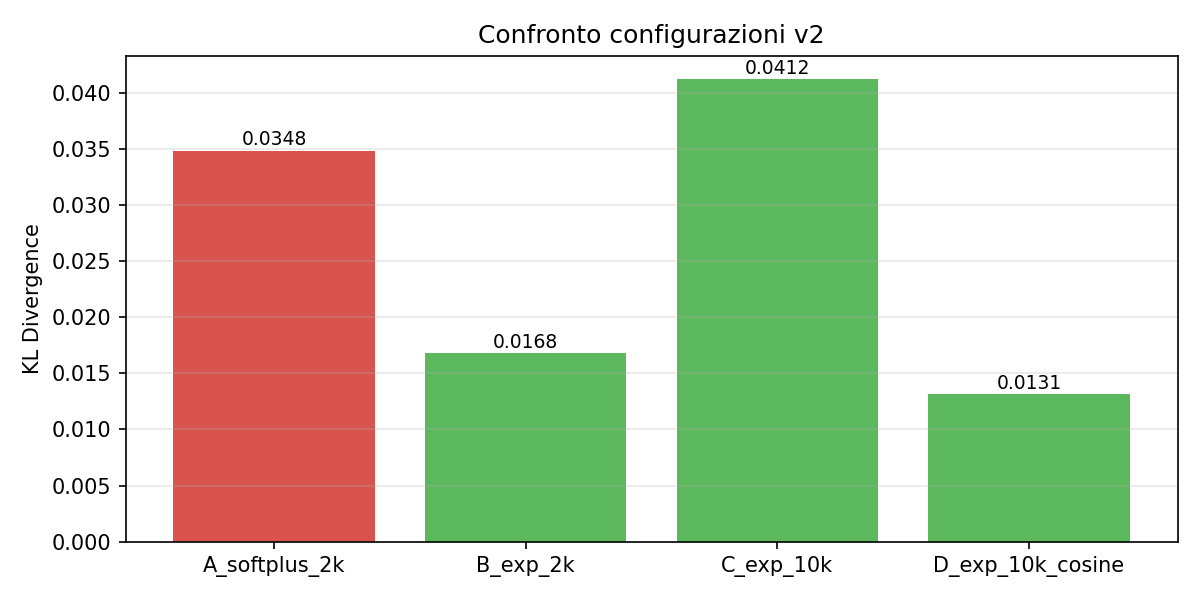
\includegraphics[width=0.85\textwidth]{../plots/v2_comparison.png}
\caption{Confronto KL tra le configurazioni v2. Il colore rosso indica \texttt{softplus}, verde indica \texttt{exp}.}
\label{fig:v2_comparison}
\end{figure}

\begin{figure}[H]
\centering
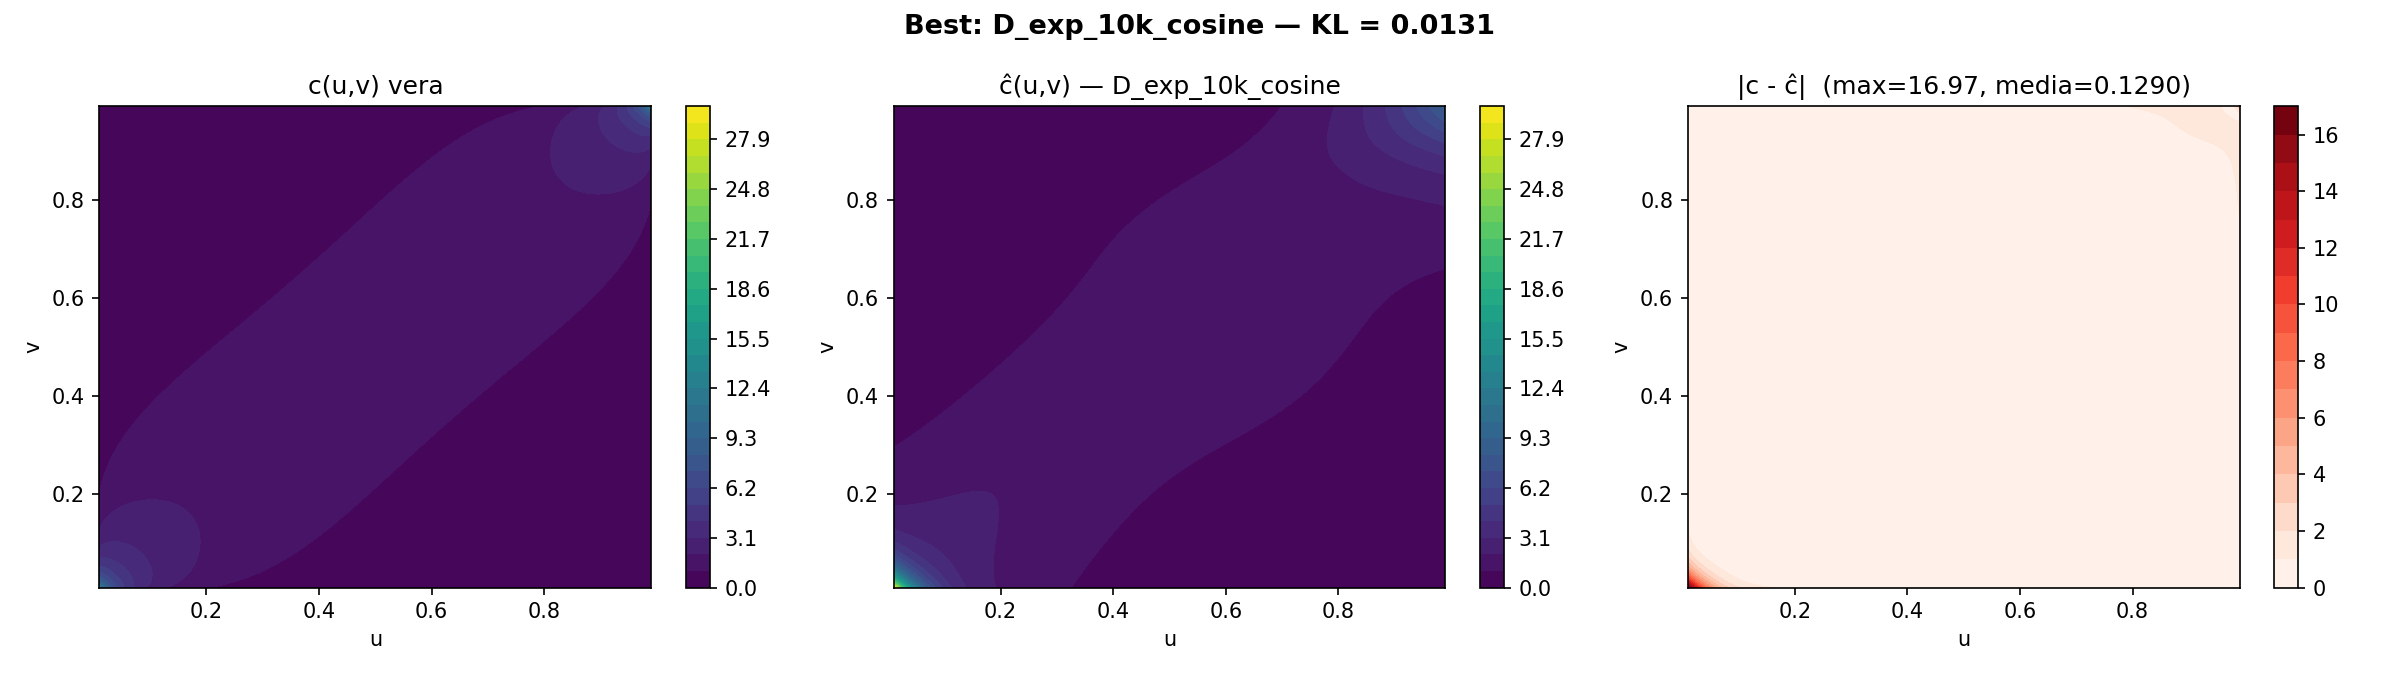
\includegraphics[width=\textwidth]{../plots/v2_best_confronto.png}
\caption{Miglior configurazione v2: confronto contour 2D tra densità vera e stimata.}
\label{fig:v2_best_confronto}
\end{figure}

\begin{figure}[H]
\centering
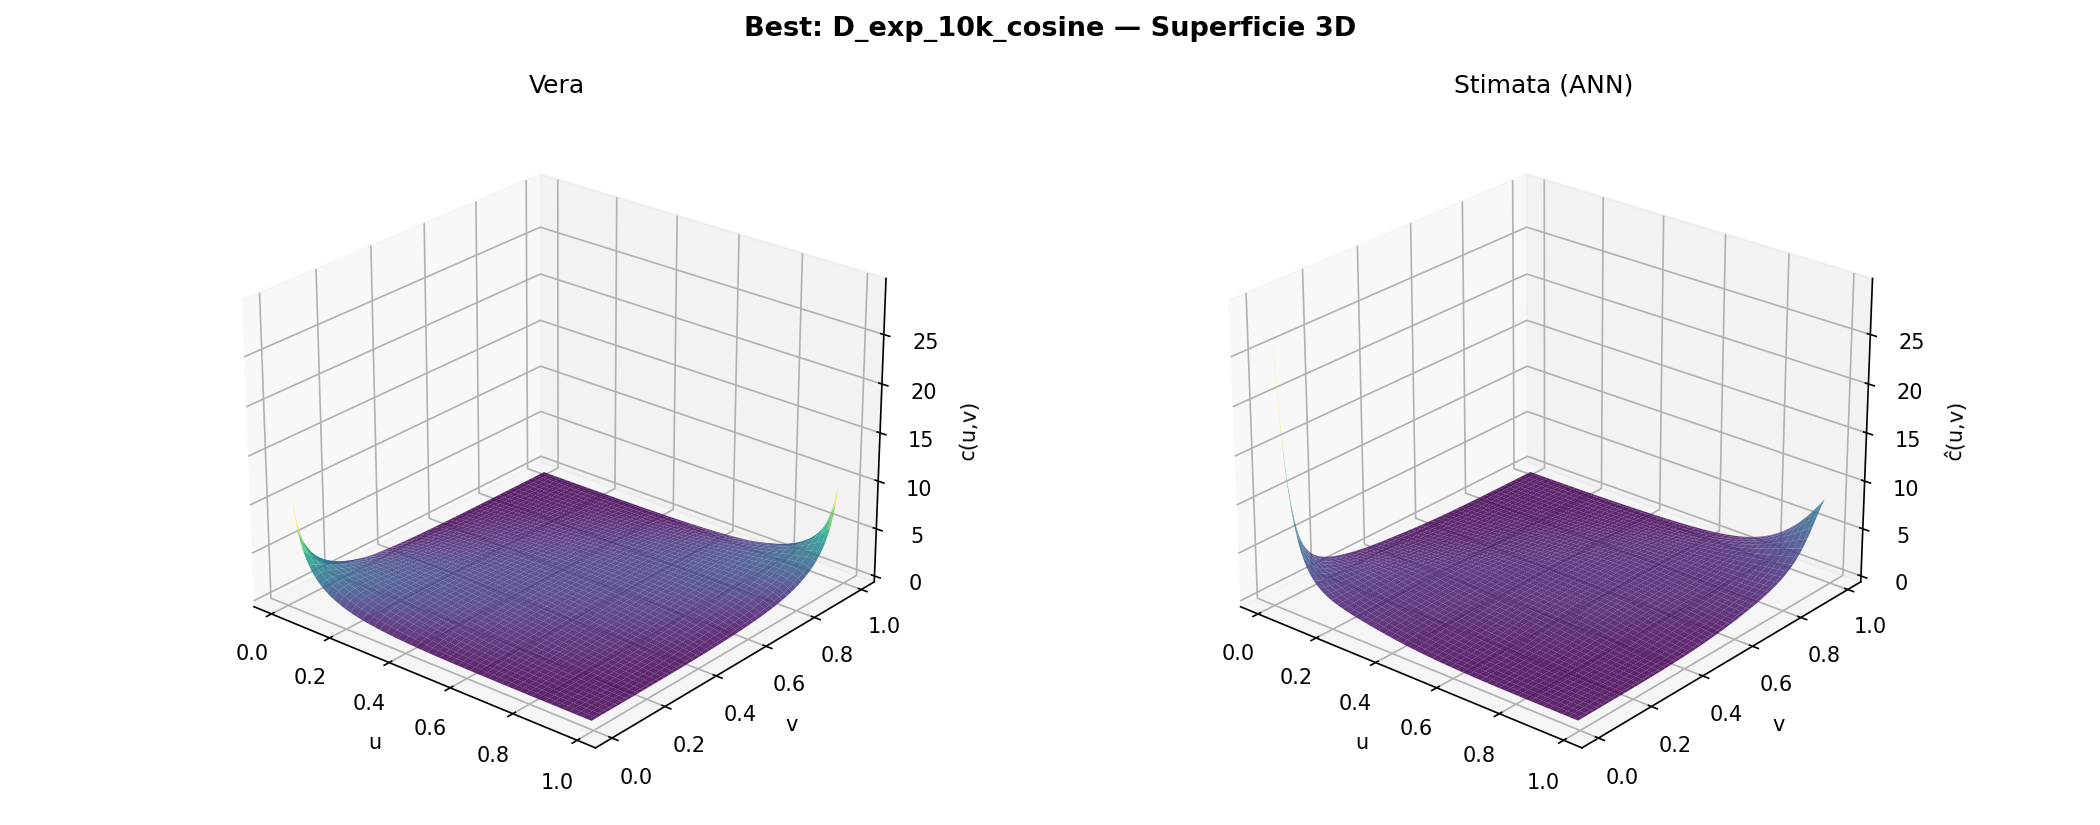
\includegraphics[width=0.85\textwidth]{../plots/v2_best_3d.png}
\caption{Miglior configurazione v2: superfici 3D. L'output \texttt{exp} riesce a raggiungere valori più alti ai picchi, ma introduce artefatti.}
\label{fig:v2_best_3d}
\end{figure}

\subsection{Analisi}

L'output \texttt{exp} riduce la KL da $0.035$ (softplus) a $0.017$ (exp, $N = 2000$), confermando che la maggiore espressività aiuta. Tuttavia introduce un problema critico: l'\textbf{errore massimo esplode} da $8.6$ a $70.8$. Con pochi dati ($N = 2000$), \texttt{exp} produce picchi spuri ai bordi del dominio.

Senza cosine annealing, \texttt{exp} con $N = 10\,000$ (config C) ottiene addirittura $\text{KL} = 0.041$, peggiore del softplus: il training è instabile e il modello converge a un minimo locale scadente. Il cosine annealing (config D) stabilizza l'ottimizzazione e raggiunge $\text{KL} = 0.013$, il miglior risultato di questo esperimento, ma con $\text{err\_max} = 17.0$ --- il doppio del softplus.

\textbf{Lezione appresa:} \texttt{exp} è più espressivo ma intrinsecamente instabile. Il cosine annealing è essenziale per \texttt{exp}, ma non risolve il problema ai bordi.

% =========================================================================
\section{Esperimento 4: Gradient clipping}
% =========================================================================

\subsection{Motivazione}

Il gradient clipping limita la norma del gradiente a un valore massimo, prevenendo aggiornamenti troppo grandi che causano instabilità con l'attivazione \texttt{exp}. Testiamo anche l'effetto di dataset molto più grandi ($N = 50\,000$) e reti più larghe ($256 \times 4$), sfruttando la GPU disponibile.

\subsection{Setup}

\begin{center}
\begin{tabular}{llcccc}
\toprule
\textbf{Config} & \textbf{Output} & $\boldsymbol{N}$ & \textbf{Arch.} & \textbf{clip} & \textbf{Sched.} \\
\midrule
baseline\_softplus & softplus & 2\,000  & $128 \times 3$ & --- & --- \\
exp\_clip\_10k     & exp      & 10\,000 & $128 \times 3$ & 1.0 & cosine \\
exp\_clip\_50k     & exp      & 50\,000 & $128 \times 3$ & 1.0 & cosine \\
exp\_wide\_50k     & exp      & 50\,000 & $256 \times 4$ & 1.0 & cosine \\
\bottomrule
\end{tabular}
\end{center}

Tutte le configurazioni: $\lambda = 10$, 10\,000 epoche, griglia integrale $100 \times 100$ (tranne baseline: $50 \times 50$).

\subsection{Risultati}

\begin{center}
\begin{tabular}{lcccc}
\toprule
\textbf{Config} & $\boldsymbol{D_\mathrm{KL}}$ & $\boldsymbol{\iint \hat{c}}$ & \textbf{err\_max} & \textbf{err\_mean} \\
\midrule
baseline\_softplus & 0.0328 & 1.046 &   9.80 & 0.209 \\
exp\_clip\_10k     & \textbf{0.0107} & 1.045 & 132.62 & 0.107 \\
exp\_clip\_50k     & \textbf{0.0107} & 1.046 & 114.19 & 0.100 \\
exp\_wide\_50k     & 0.0133 & 1.046 &  98.54 & 0.109 \\
\bottomrule
\end{tabular}
\end{center}

\begin{figure}[H]
\centering
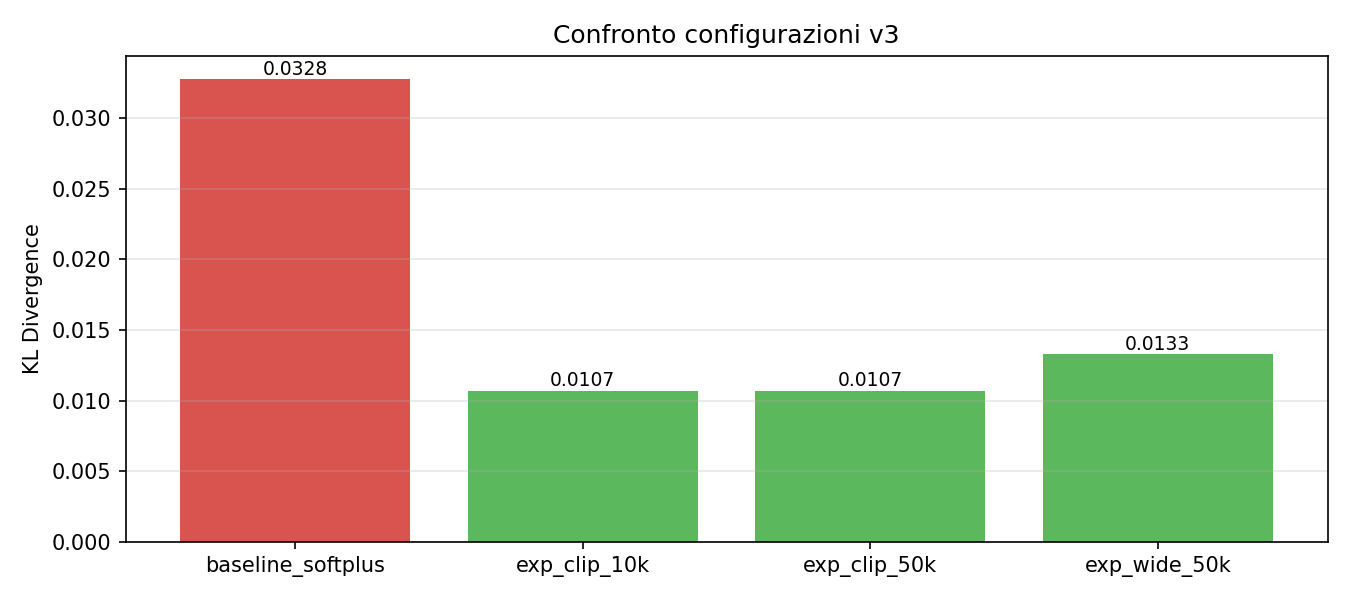
\includegraphics[width=0.85\textwidth]{../plots/v3_comparison.png}
\caption{Confronto KL tra le configurazioni v3. Il gradient clipping e più dati riducono la KL, ma l'errore massimo resta elevato.}
\label{fig:v3_comparison}
\end{figure}

\begin{figure}[H]
\centering
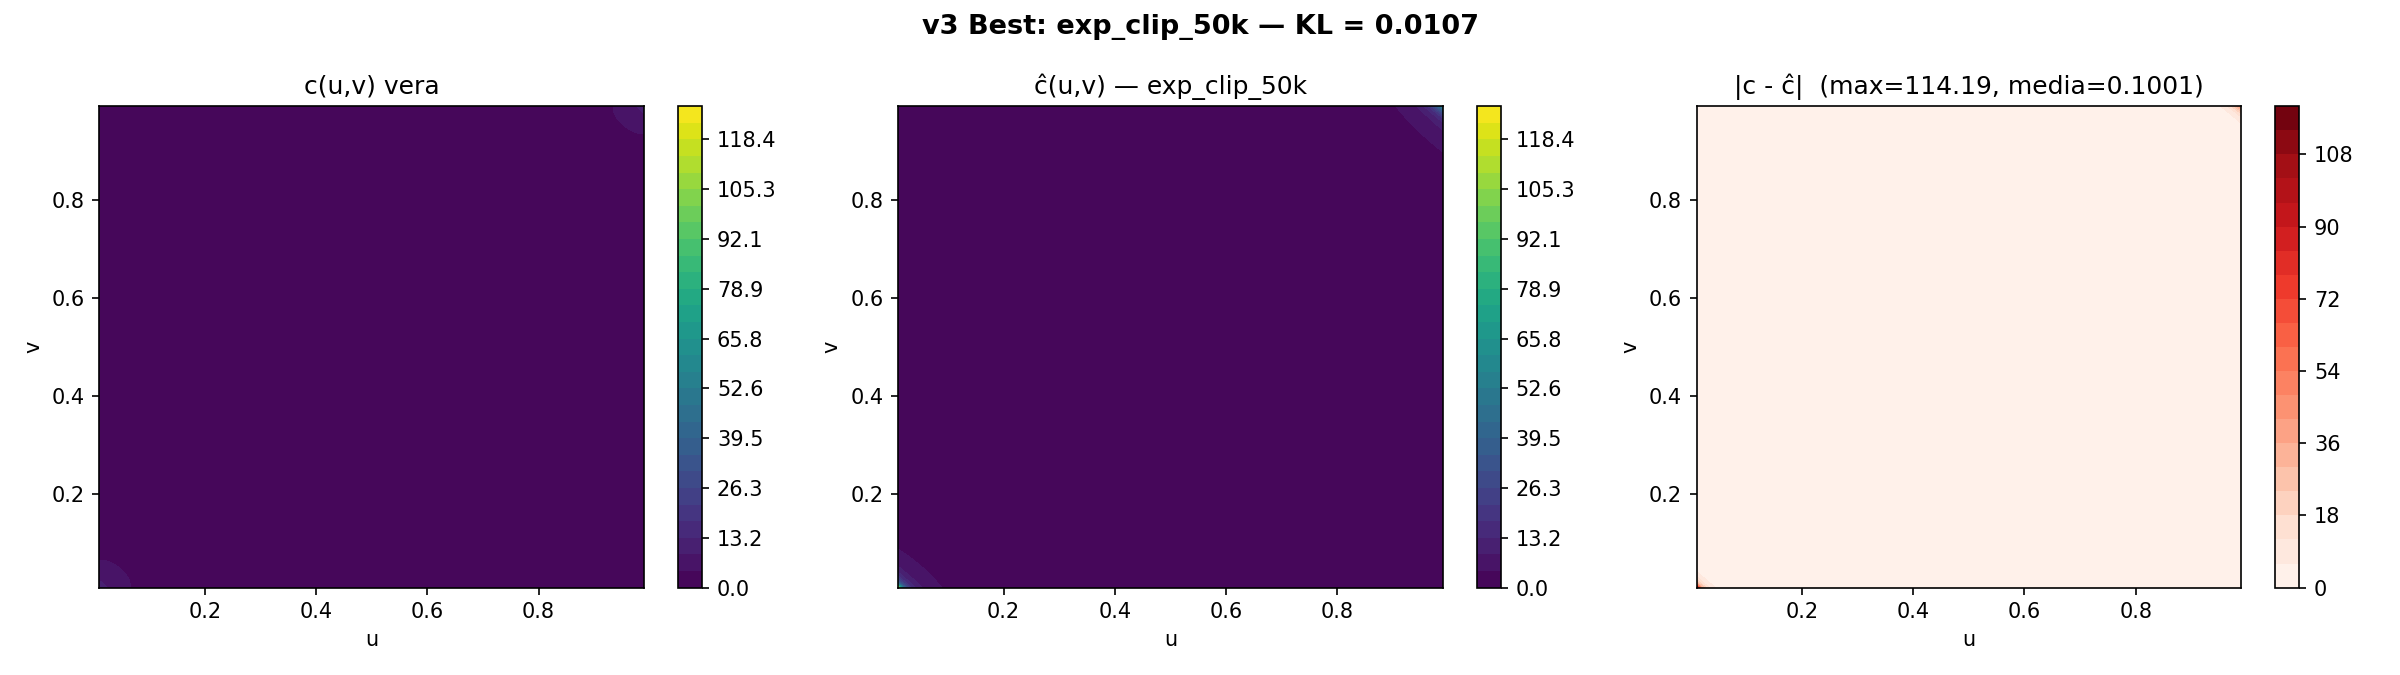
\includegraphics[width=\textwidth]{../plots/v3_best_confronto.png}
\caption{Miglior configurazione v3: il contour mostra una buona corrispondenza qualitativa, ma l'errore massimo è concentrato agli angoli.}
\label{fig:v3_best_confronto}
\end{figure}

\begin{figure}[H]
\centering
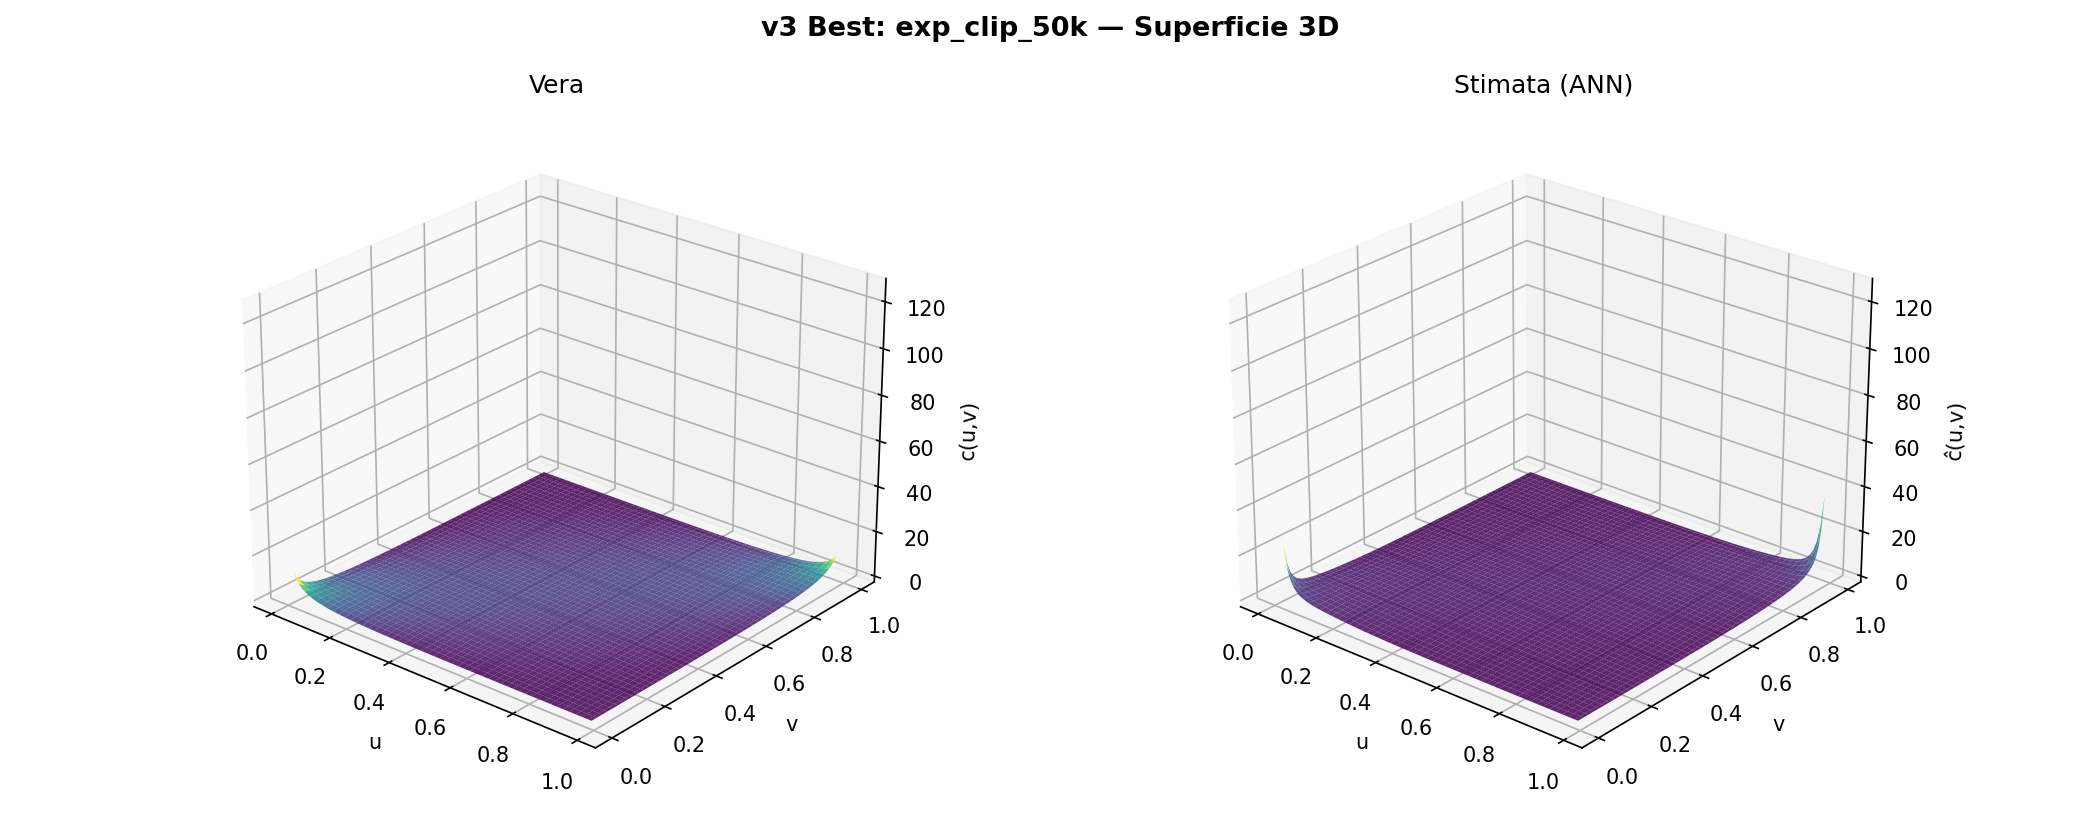
\includegraphics[width=0.85\textwidth]{../plots/v3_best_3d.png}
\caption{Miglior configurazione v3: superfici 3D. La rete raggiunge picchi più alti della vera copula (overshooting) a causa dell'instabilità di \texttt{exp}.}
\label{fig:v3_best_3d}
\end{figure}

\begin{figure}[H]
\centering
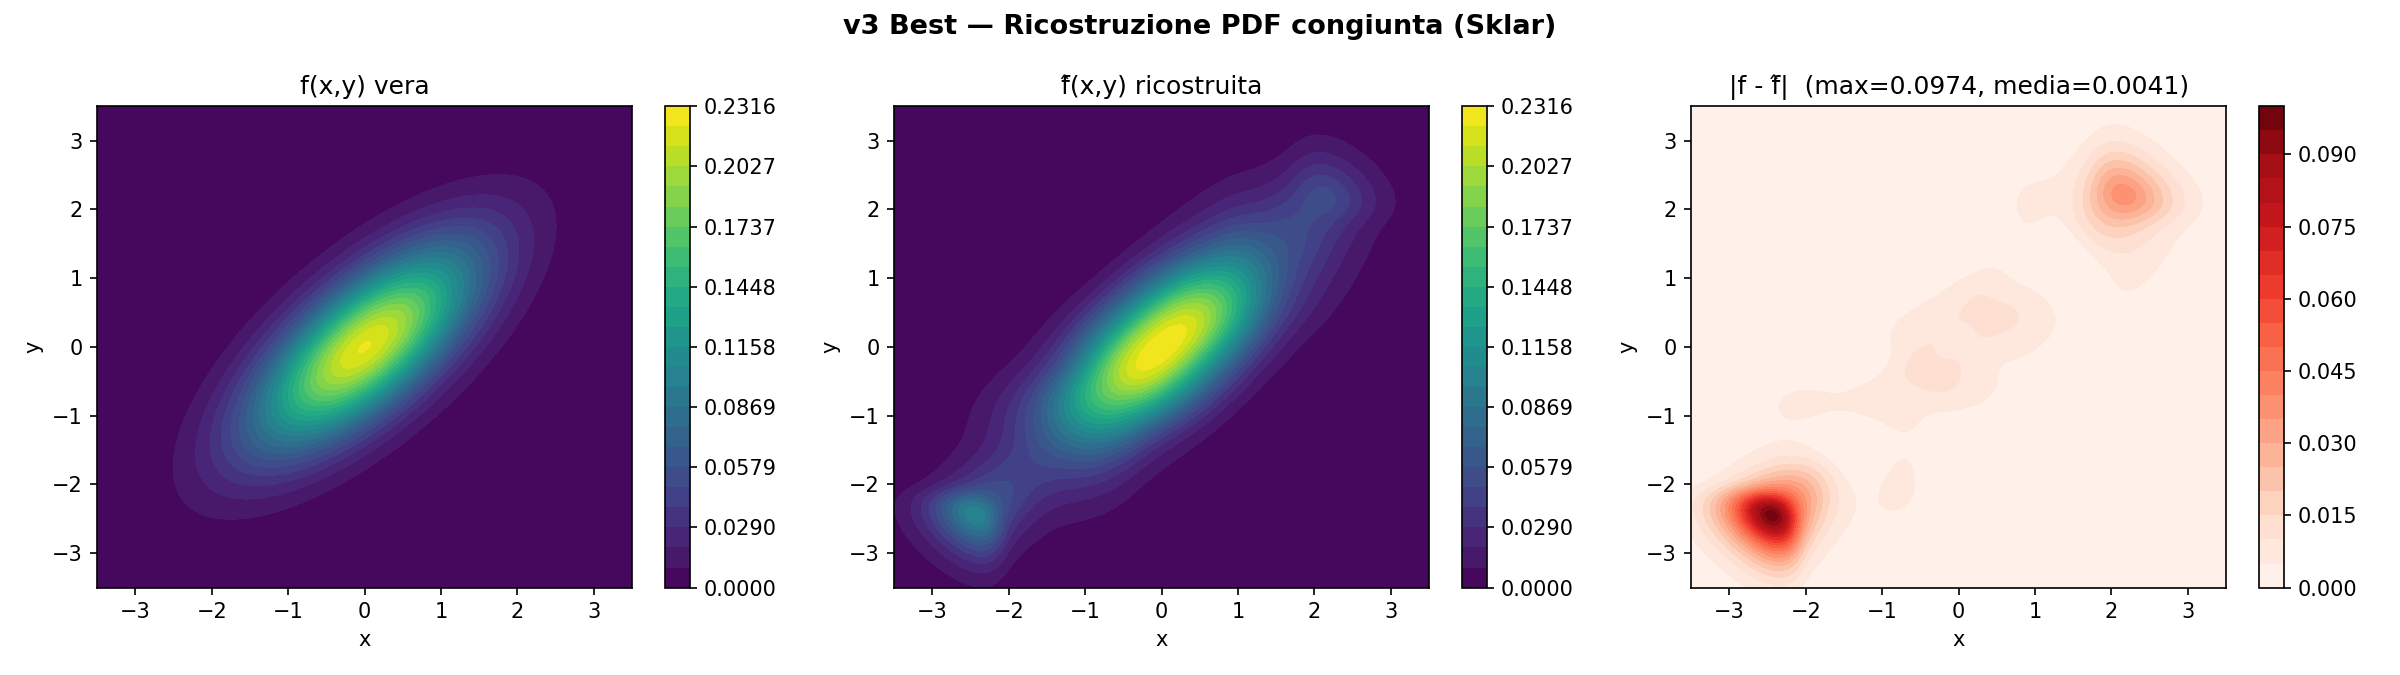
\includegraphics[width=\textwidth]{../plots/v3_best_joint.png}
\caption{Miglior configurazione v3: ricostruzione PDF congiunta. L'overshooting della copula ai bordi si propaga alla ricostruzione, causando errori elevati nonostante la KL apparentemente bassa.}
\label{fig:v3_best_joint}
\end{figure}

\subsection{Analisi}

Il gradient clipping (max\_norm $= 1.0$) combinato con cosine annealing raggiunge $\text{KL} = 0.0107$ con $N = 10\,000$ e $50\,000$, un miglioramento rispetto all'Esperimento~3. Tuttavia i risultati rivelano un pattern critico:

\begin{itemize}
    \item La KL migliora con più dati e gradient clipping (da $0.033$ a $0.011$).
    \item Ma l'\textbf{errore massimo esplode}: $\text{err\_max} = 132.6$ (10k) e $114.2$ (50k), un ordine di grandezza peggiore del softplus ($9.8$).
    \item La rete più larga ($256 \times 4$, 198\,401 parametri) non migliora: $\text{KL} = 0.013$, peggiore del $128 \times 3$. Più parametri amplificano l'instabilità.
    \item Il gradient clipping riduce l'err\_max da $\sim 200$ (senza clip, Esp.~3) a $\sim 100$--$130$, ma resta inaccettabile.
\end{itemize}

\textbf{Conclusione:} il gradient clipping è una \emph{patch} insufficiente. Il problema è strutturale: la rete opera nello spazio sbagliato.

% =========================================================================
\section{Il problema fondamentale}
% =========================================================================

La copula gaussiana con $\rho = 0.7$ ha densità:
\[
c(u,v) = \frac{1}{\sqrt{1-\rho^2}} \exp\!\left(-\frac{\rho^2(x^2+y^2) - 2\rho\, x\, y}{2(1-\rho^2)}\right), \qquad x = \Phi^{-1}(u),\; y = \Phi^{-1}(v)
\]

Quando $u \to 0$ o $u \to 1$, la quantile function $\Phi^{-1}(u) \to \mp\infty$ e la densità della copula \textbf{diverge} lungo la diagonale concordante. Nella griglia di valutazione ($\varepsilon = 0.01$), $c(0.01, 0.01) \approx 13$.

Questo crea un dilemma per la rete neurale:
\begin{itemize}
    \item \texttt{softplus}$(z) \approx z$ per $z \gg 0$: cresce linearmente, non può raggiungere valori alti senza logit enormi. \textbf{Risultato: sottostima i picchi.}
    \item \texttt{exp}$(z) = e^z$: può raggiungere qualsiasi valore, ma è ipersensibile. Anche piccoli errori nel logit producono grandi errori nell'output. \textbf{Risultato: instabilità e overshooting.}
\end{itemize}

Il punto chiave è che la rete lavora nello spazio $(u,v) \in [0,1]^2$, dove la copula presenta variazioni estreme su regioni minuscole vicino agli angoli. La rete deve ``imparare'' la divergenza $\Phi^{-1}$ implicitamente nei pesi, il che è inefficiente.

% =========================================================================
\section{Esperimento 5: Trasformazione degli input}
% =========================================================================

\subsection{Idea}

Invece di dare $(u,v)$ direttamente alla rete, le forniamo
\[
(x, y) = \bigl(\Phi^{-1}(u),\; \Phi^{-1}(v)\bigr) \in \mathbb{R}^2
\]

In questo spazio trasformato, la densità della copula gaussiana diventa:
\[
c\bigl(\Phi(x), \Phi(y)\bigr) = \frac{1}{\sqrt{1-\rho^2}} \exp\!\left(-\frac{\rho^2(x^2+y^2) - 2\rho\, x\, y}{2(1-\rho^2)}\right)
\]
che è una funzione \textbf{liscia, limitata, simile a una gaussiana riscalata} --- molto più facile da apprendere per un MLP. I punti che nel quadrato unitario si comprimono agli angoli vengono ``distesi'' nello spazio trasformato.

Nota implementativa: la trasformazione $\Phi^{-1}$ è implementata all'interno del modello, prima dello strato di input, tramite \texttt{torch.erfinv}. I valori in input vengono clampati a $[10^{-4},\, 1-10^{-4}]$ per evitare divergenze numeriche.

\subsection{Setup}

\begin{center}
\begin{tabular}{llcccccc}
\toprule
\textbf{Config} & \textbf{Output} & $\boldsymbol{N}$ & \textbf{$\Phi^{-1}$} & \textbf{Ep.} & \textbf{Sched.} & \textbf{clip} \\
\midrule
ref\_no\_transform  & softplus & 2\,000  & No & 5\,000 & --- & --- \\
transform\_sp\_2k   & softplus & 2\,000  & Sì & 5\,000 & --- & --- \\
transform\_sp\_10k  & softplus & 10\,000 & Sì & 10\,000 & cosine & --- \\
transform\_exp\_10k & exp      & 10\,000 & Sì & 10\,000 & cosine & 1.0 \\
\bottomrule
\end{tabular}
\end{center}

Tutte le configurazioni: architettura $128 \times 3$, $\lambda = 10$.

\subsection{Risultati}

\begin{center}
\begin{tabular}{lccccc}
\toprule
\textbf{Config} & $\boldsymbol{D_\mathrm{KL}}$ & $\boldsymbol{\iint \hat{c}}$ & \textbf{err\_max} & \textbf{err\_mean} & $\boldsymbol{L_1}$ \textbf{joint} \\
\midrule
ref\_no\_transform  & 0.0091 & 1.047 & 6.06  & 0.117 & 0.136 \\
transform\_sp\_2k   & 0.0066 & 1.045 & 6.25  & 0.099 & 0.128 \\
transform\_sp\_10k  & \textbf{0.0032} & 1.045 & 8.09  & 0.094 & 0.204 \\
transform\_exp\_10k & 0.0190 & 1.020 & 243.6 & 0.133 & $>10^{16}$ \\
\bottomrule
\end{tabular}
\end{center}

\begin{figure}[H]
\centering
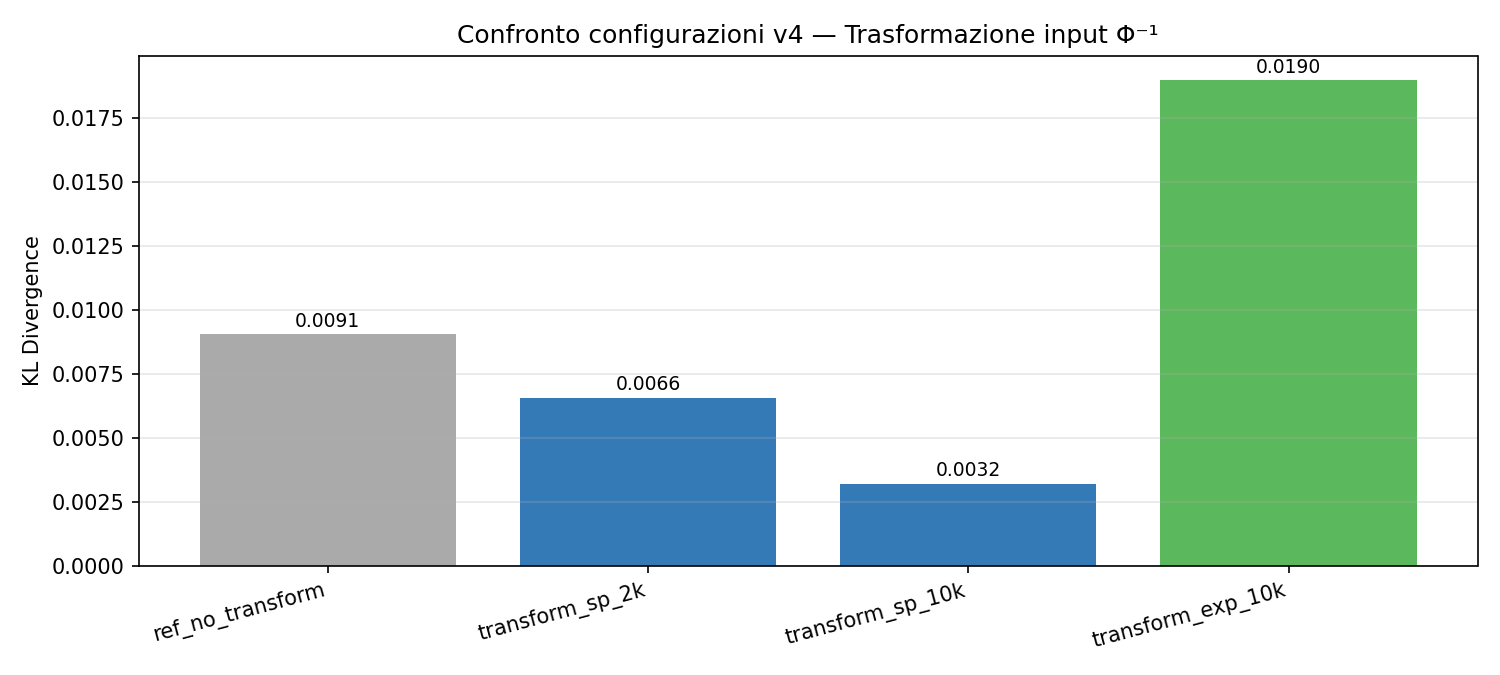
\includegraphics[width=0.85\textwidth]{../plots/v4_comparison.png}
\caption{Confronto KL --- Esperimento 5. Le barre blu indicano \texttt{softplus} con trasformazione, grigio senza trasformazione, verde \texttt{exp} con trasformazione.}
\label{fig:v4_comparison}
\end{figure}

\begin{figure}[H]
\centering
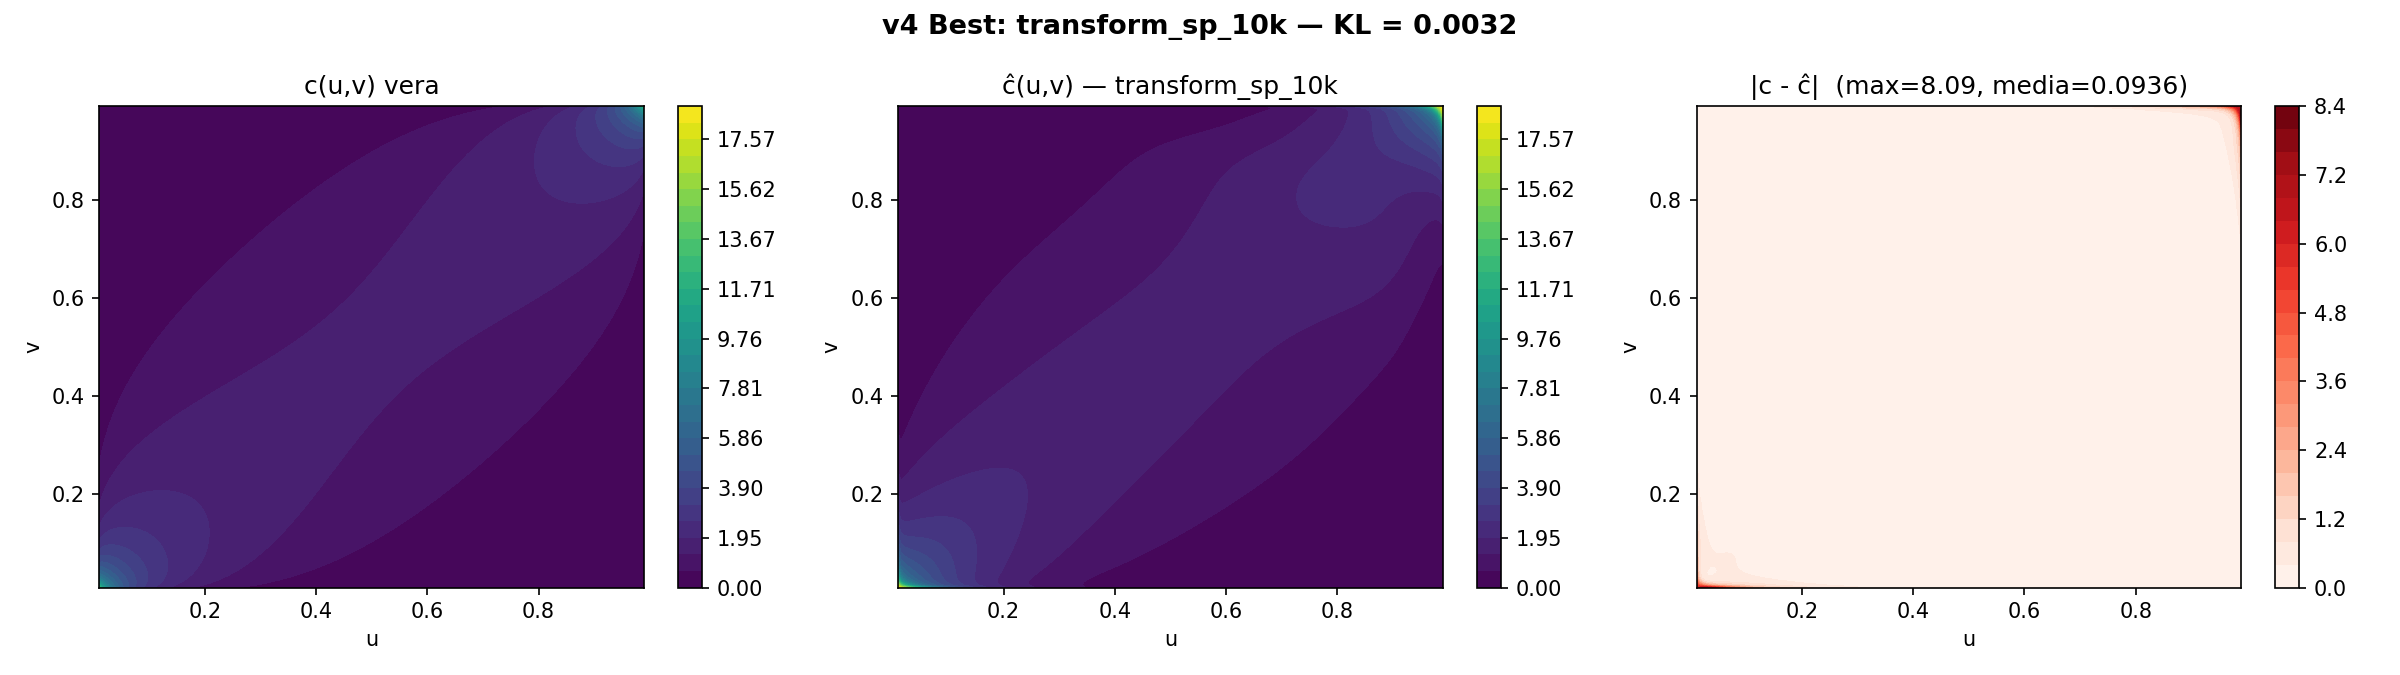
\includegraphics[width=\textwidth]{../plots/v4_best_confronto.png}
\caption{Miglior configurazione v4 (\texttt{transform\_sp\_10k}): confronto contour 2D. La forma è catturata molto meglio rispetto ai checkpoint precedenti, specialmente nella regione centrale.}
\label{fig:v4_best_confronto}
\end{figure}

\begin{figure}[H]
\centering
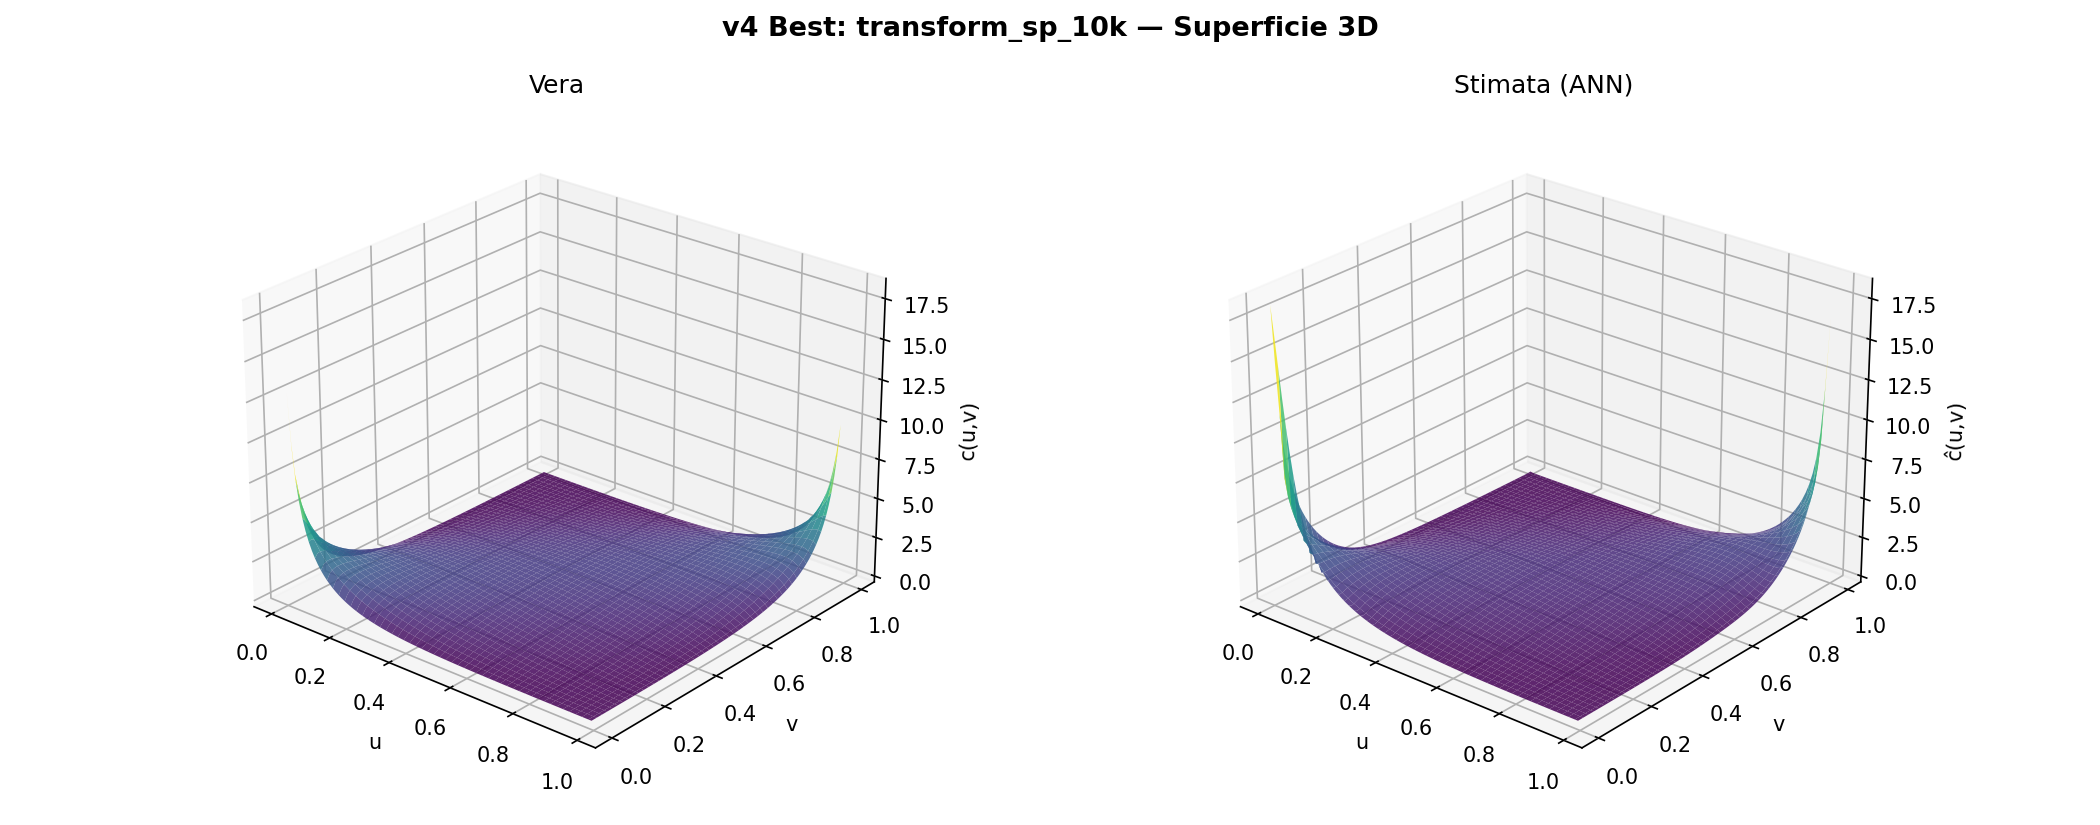
\includegraphics[width=0.85\textwidth]{../plots/v4_best_3d.png}
\caption{Miglior configurazione v4: superfici 3D. I picchi agli angoli sono ancora sottostimati (\texttt{softplus} non può raggiungere il vero valore $\sim 13$), ma la forma complessiva è molto più accurata.}
\label{fig:v4_best_3d}
\end{figure}

\begin{figure}[H]
\centering
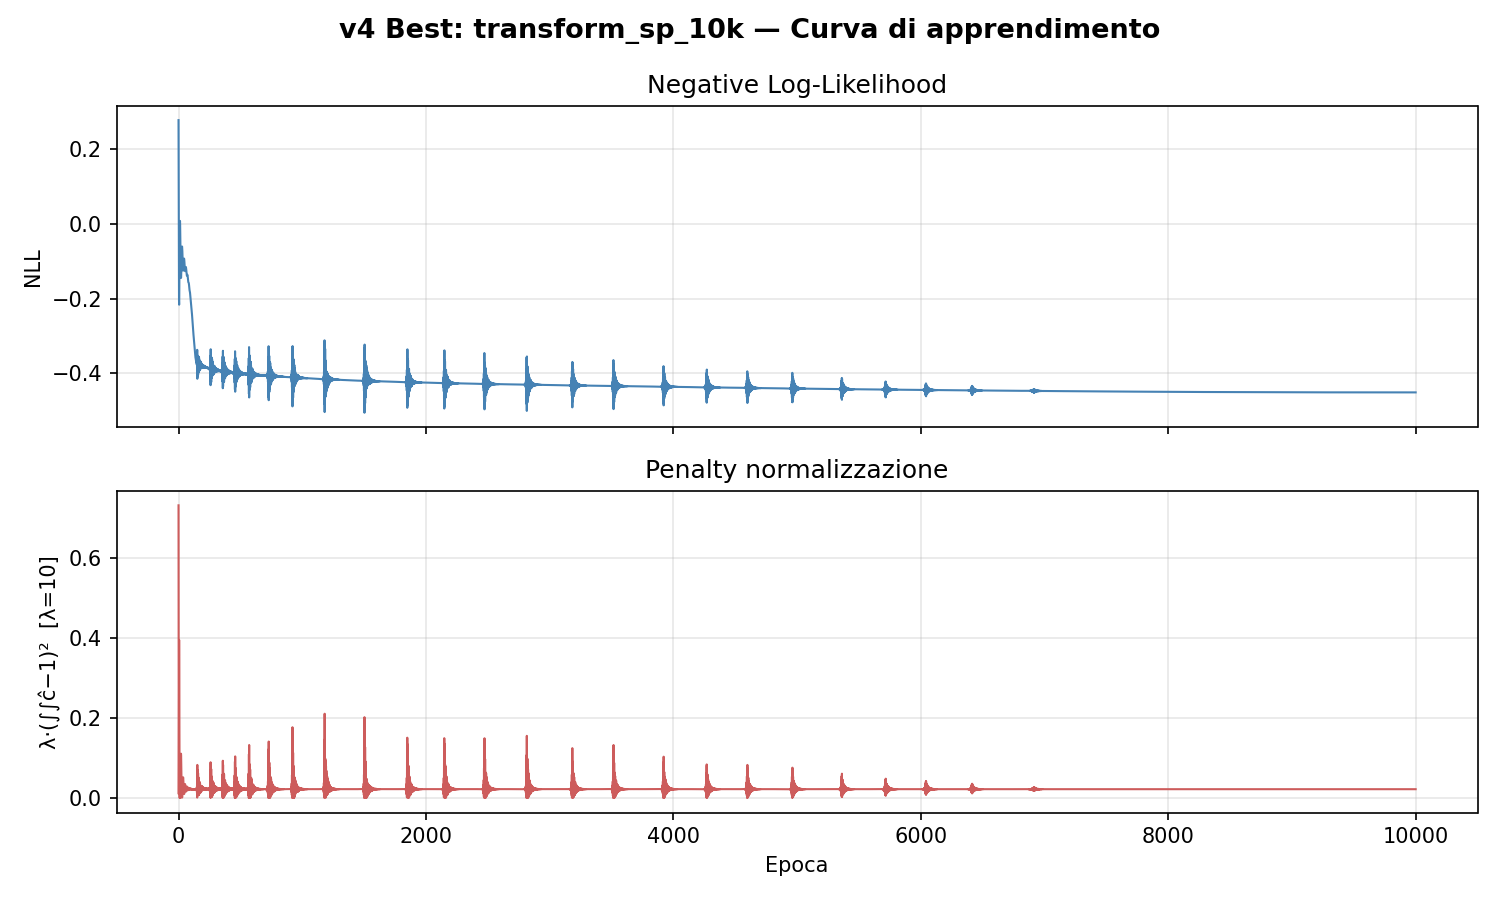
\includegraphics[width=0.85\textwidth]{../plots/v4_best_learning.png}
\caption{Curva di apprendimento --- \texttt{transform\_sp\_10k}. La NLL scende più rapidamente e raggiunge valori più bassi ($\approx -0.45$) rispetto alle configurazioni senza trasformazione ($\approx -0.40$).}
\label{fig:v4_best_learning}
\end{figure}

\begin{figure}[H]
\centering
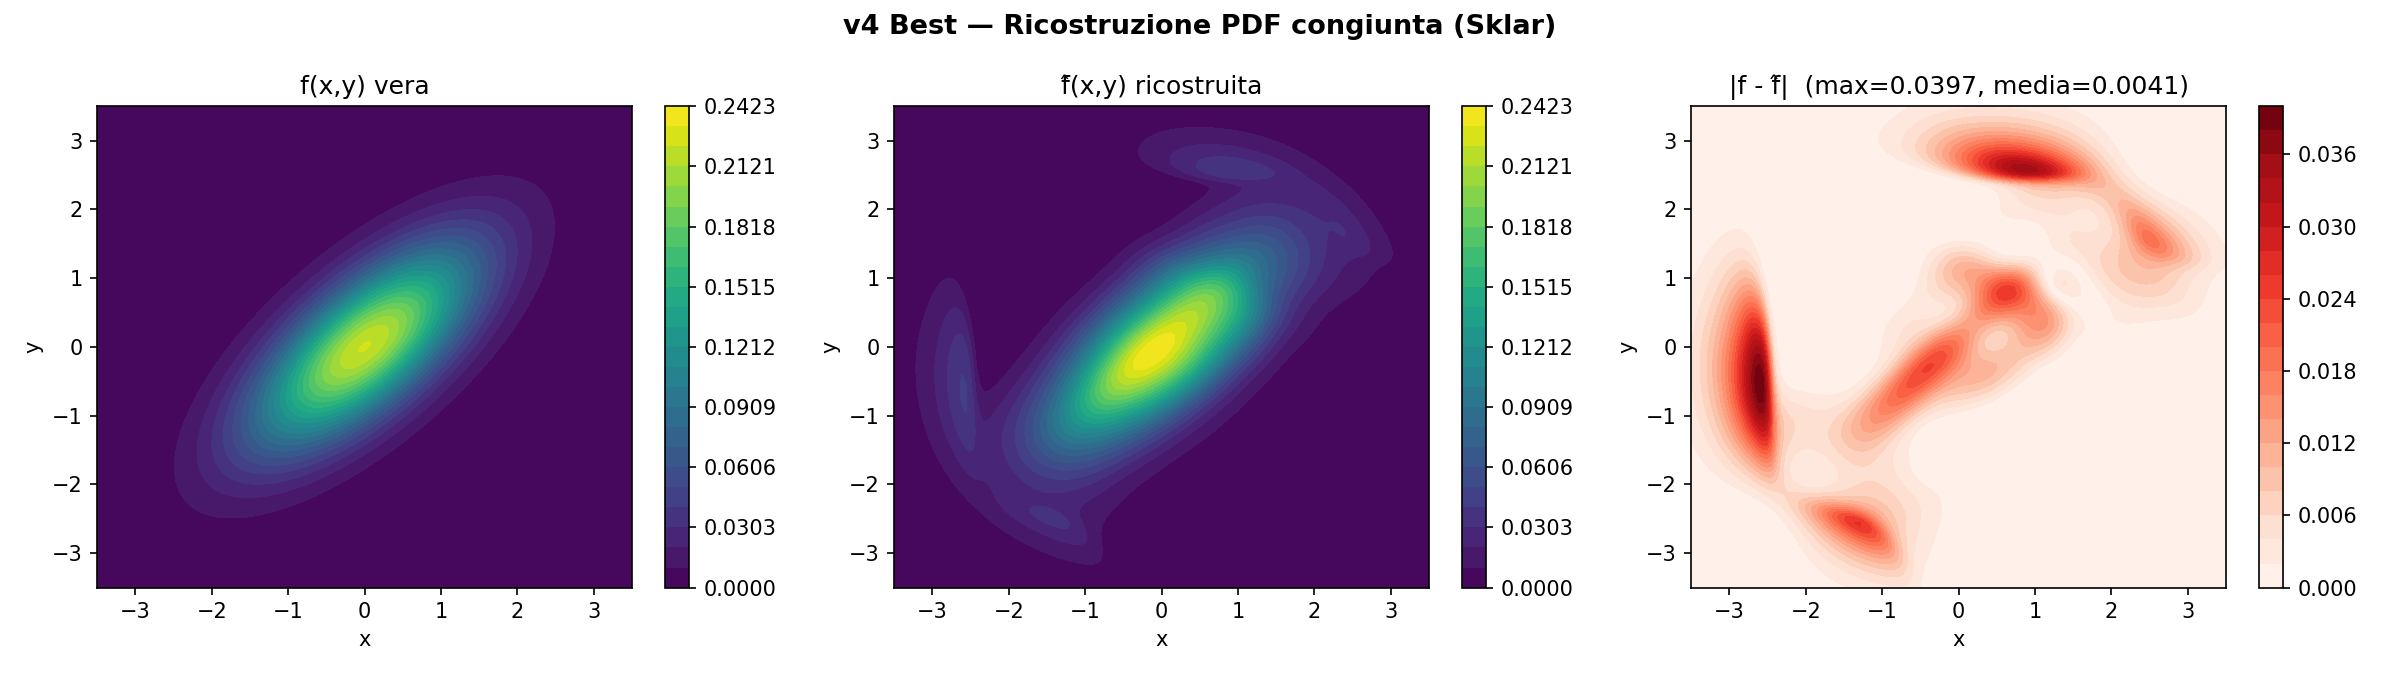
\includegraphics[width=\textwidth]{../plots/v4_best_joint.png}
\caption{Ricostruzione PDF congiunta via Sklar per la configurazione \texttt{transform\_sp\_10k}. La ricostruzione è qualitativamente eccellente.}
\label{fig:v4_best_joint}
\end{figure}

\subsection{Analisi}

La trasformazione degli input è il singolo miglioramento più efficace tra tutti quelli testati:

\begin{itemize}
    \item \textbf{A parità di tutto il resto} (stessa rete, stessi dati, stesse epoche), la trasformazione riduce la KL da $0.0091$ a $0.0066$ ($-27\%$).
    \item \textbf{Con più dati} ($N = 10\,000$) e cosine annealing, la KL scende a $\mathbf{0.0032}$ --- il miglior risultato ottenuto finora, quasi tre volte meglio del checkpoint 1 ($0.010$).
    \item L'\texttt{exp} con trasformazione \textbf{diverge completamente}: nello spazio trasformato gli input $\Phi^{-1}(u)$ possono essere grandi ($|\Phi^{-1}(0.01)| \approx 2.33$), e l'attivazione \texttt{exp} amplifica ulteriormente. La combinazione è catastrofica.
    \item \texttt{softplus} con trasformazione è la combinazione vincente: stabile, accurata, e significativamente migliore del baseline.
\end{itemize}

\textbf{Perché funziona:} la trasformazione $\Phi^{-1}$ ``distende'' le regioni compresse agli angoli di $[0,1]^2$, dove la copula cambia rapidamente. La rete non deve più imparare implicitamente la divergenza $\Phi^{-1}$ nei pesi --- le viene fornita come pre-processing. Il risultato è una funzione target molto più liscia e facile da apprendere.

% =========================================================================
\section{Ablation study: isolamento dei contributi}
% =========================================================================

Gli Esperimenti 3--5 hanno introdotto simultaneamente più modifiche (attivazione, trasformazione, $N$, scheduler). Per quantificare il contributo di ciascun fattore, conduciamo un \textbf{ablation study} con design fattoriale: prendiamo le due baseline del Checkpoint 1 (naive e best) e applichiamo in isolamento le due modifiche più promettenti:
\begin{itemize}
    \item Trasformazione degli input $\Phi^{-1}$
    \item Aumento dei campioni ($N = 10\,000$ vs.\ $2\,000$)
\end{itemize}
Tutto il resto è identico al Checkpoint 1: \texttt{softplus}, 5\,000 epoche, nessun scheduler, nessun gradient clipping.

\subsection{Risultati}

\begin{center}
\begin{tabular}{llccccccc}
\toprule
\textbf{Gruppo} & \textbf{Config} & $\boldsymbol{N}$ & $\boldsymbol{\Phi^{-1}}$ & $\boldsymbol{D_\mathrm{KL}}$ & \textbf{err\_max} & \textbf{err\_mean} & $\boldsymbol{L_1}$ \textbf{joint} & $\boldsymbol{\Delta}$\textbf{KL} \\
\midrule
\multirow{4}{*}{Naive}
 & baseline         & 2k  & No & 0.0237 & 10.40 & 0.140 & 0.162 & --- \\
 & $+\Phi^{-1}$     & 2k  & Sì & 0.0061 &  7.66 & 0.079 & 0.091 & $-74\%$ \\
 & $+10\text{k}$    & 10k & No & 0.0256 & 10.25 & 0.160 & 0.181 & $+8\%$ \\
 & $+\Phi^{-1}+10\text{k}$ & 10k & Sì & \textbf{0.0039} & 6.88 & 0.070 & 0.081 & $-84\%$ \\
\midrule
\multirow{4}{*}{Best}
 & baseline         & 2k  & No & 0.0105 &  3.82 & 0.129 & 0.147 & --- \\
 & $+\Phi^{-1}$     & 2k  & Sì & 0.0062 &  6.26 & 0.095 & 0.126 & $-41\%$ \\
 & $+10\text{k}$    & 10k & No & 0.0050 &  5.48 & 0.100 & 0.118 & $-52\%$ \\
 & $+\Phi^{-1}+10\text{k}$ & 10k & Sì & \textbf{0.0034} & 4.66 & 0.093 & 0.115 & $-68\%$ \\
\bottomrule
\end{tabular}
\end{center}

\begin{figure}[H]
\centering
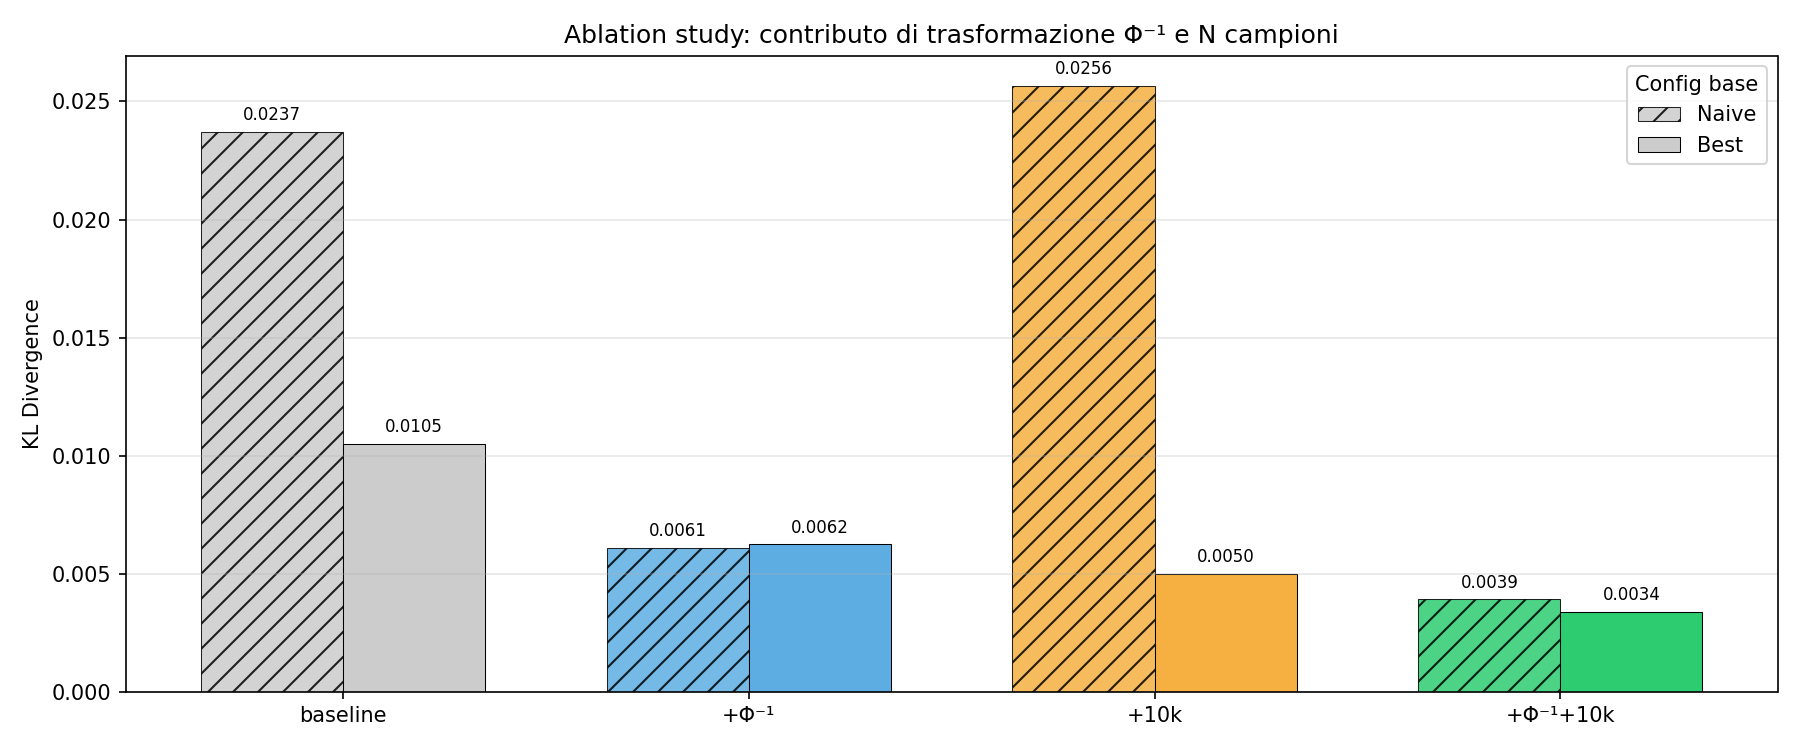
\includegraphics[width=\textwidth]{../plots/ablation_comparison.png}
\caption{Ablation study: contributo isolato di ciascun fattore. Le barre tratteggiate sono il gruppo Naive ($64 \times 2$, $\lambda = 100$), quelle piene il gruppo Best ($128 \times 3$, $\lambda = 10$). I colori indicano: grigio = baseline, blu = solo $\Phi^{-1}$, arancio = solo $+10$k, verde = entrambi.}
\label{fig:ablation}
\end{figure}

\begin{figure}[H]
\centering
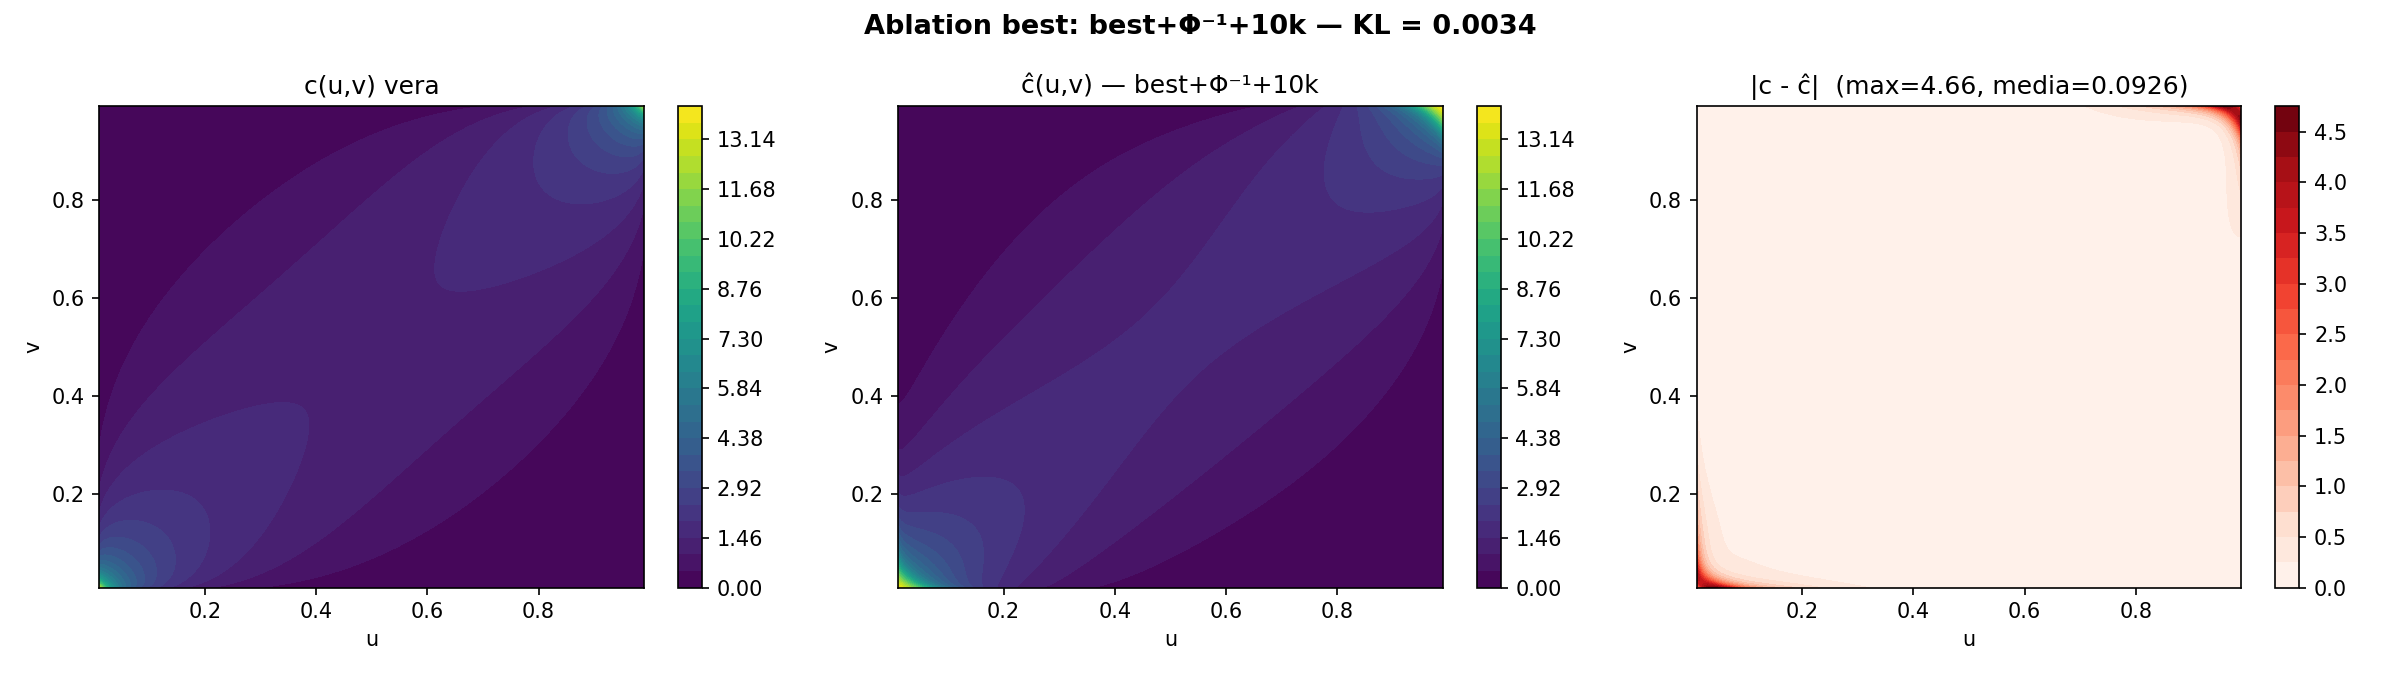
\includegraphics[width=\textwidth]{../plots/ablation_best_confronto.png}
\caption{Miglior configurazione dell'ablation study (\texttt{best}$+\Phi^{-1}+10$k): confronto contour 2D. $D_\mathrm{KL} = 0.0034$, la stima più accurata ottenuta con sole 5\,000 epoche.}
\label{fig:ablation_best_confronto}
\end{figure}

\begin{figure}[H]
\centering
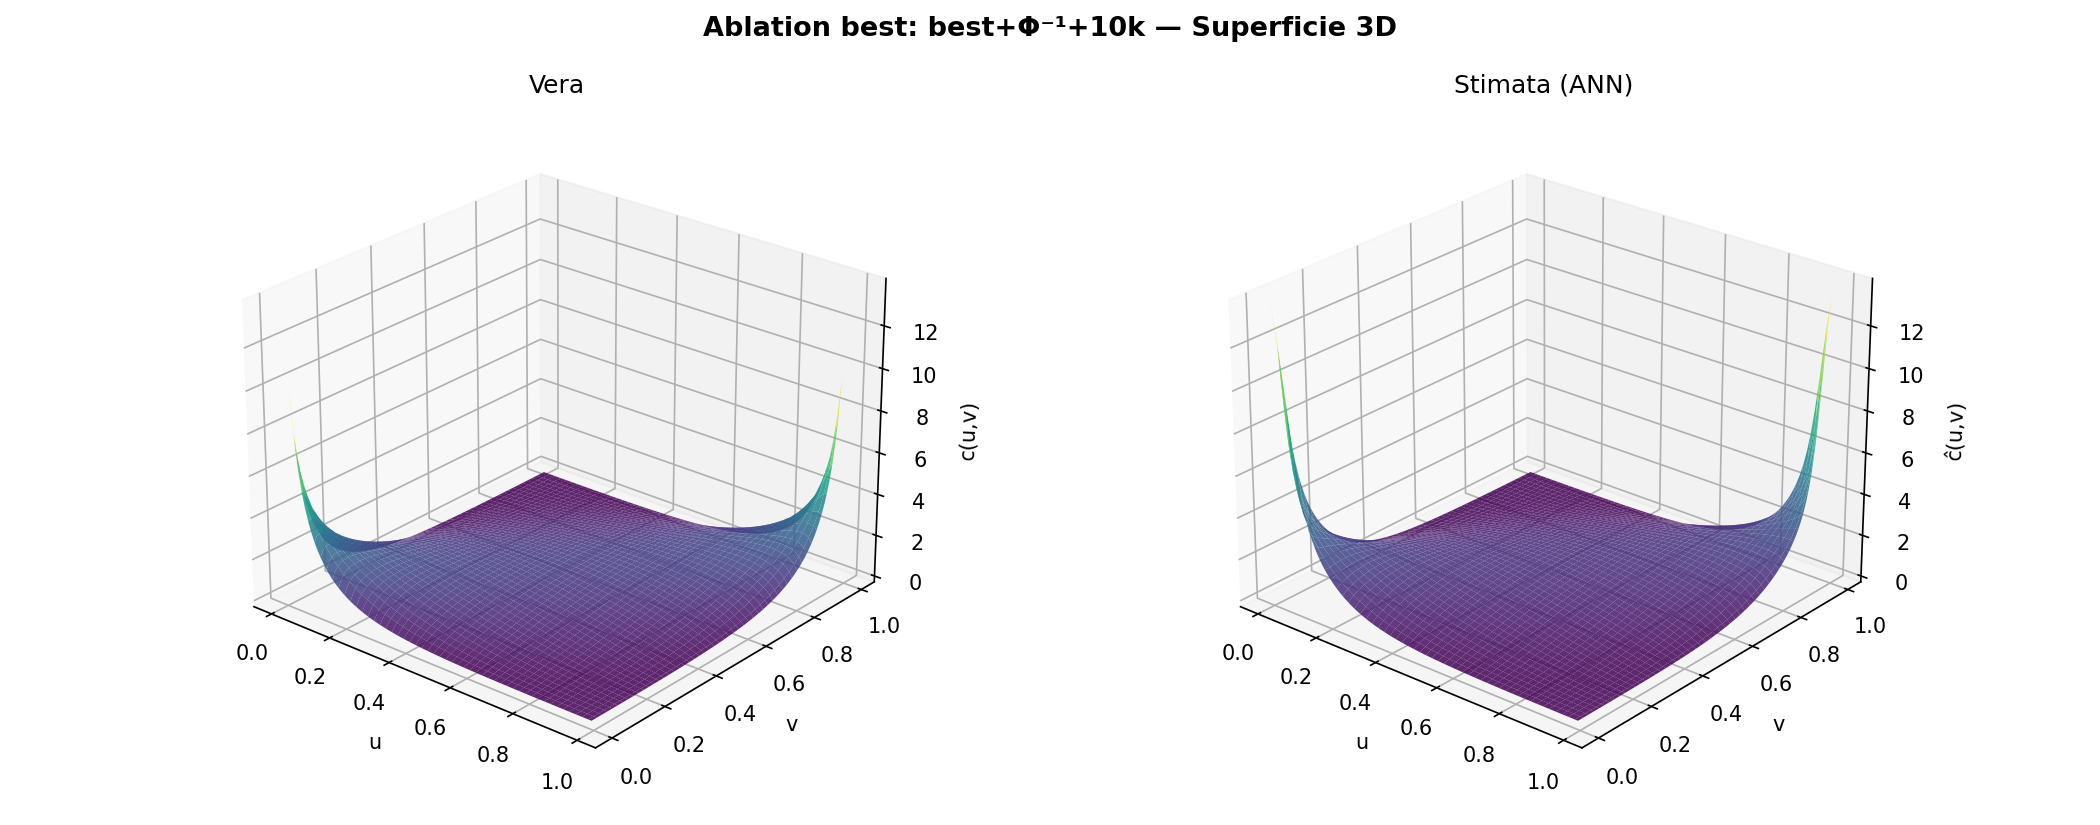
\includegraphics[width=0.85\textwidth]{../plots/ablation_best_3d.png}
\caption{Miglior configurazione dell'ablation study: superfici 3D. Confrontata con le Figure~\ref{fig:v3_best_3d} e~\ref{fig:v4_best_3d}, i picchi sono catturati meglio e senza artefatti.}
\label{fig:ablation_best_3d}
\end{figure}

\subsection{Analisi}

I risultati mostrano chiaramente la gerarchia dei fattori:

\begin{enumerate}
    \item \textbf{La trasformazione $\Phi^{-1}$ è il fattore dominante.} Sul gruppo Naive, riduce la KL del $74\%$ da sola. Risultato notevole: \texttt{naive}$+\Phi^{-1}$ ($\text{KL} = 0.006$, 4\,417 parametri) \textbf{batte} \texttt{best} senza trasformazione ($\text{KL} = 0.011$, 33\,537 parametri). La trasformazione è più impattante di $8\times$ più parametri e migliori iperparametri.

    \item \textbf{Più dati ($N = 10$k) aiutano solo con la trasformazione o con $\lambda$ basso.} Sul gruppo Naive ($\lambda = 100$), $N = 10$k peggiora leggermente la KL ($+8\%$): la penalty domina e più dati non cambiano la dinamica. Sul gruppo Best ($\lambda = 10$), $N = 10$k migliora del $52\%$. La lezione: più dati sono utili solo se il modello ha libertà di sfruttarli.

    \item \textbf{I due fattori sono complementari.} La combinazione $\Phi^{-1} + 10$k dà i risultati migliori in entrambi i gruppi, con miglioramenti additivi rispetto ai singoli fattori.
\end{enumerate}

Il miglior risultato complessivo è \texttt{best}$+\Phi^{-1}+10\text{k}$ con $\text{KL} = 0.0034$, ma \texttt{naive}$+\Phi^{-1}+10\text{k}$ ($\text{KL} = 0.0039$) è sorprendentemente vicino, suggerendo che con la trasformazione anche architetture piccole sono sufficienti.

% =========================================================================
\section{Confronto riepilogativo}
% =========================================================================

\begin{center}
\begin{tabular}{llcccc}
\toprule
\textbf{Ckp.} & \textbf{Configurazione} & $\boldsymbol{D_\mathrm{KL}}$ & \textbf{err\_max} & \textbf{err\_mean} & $\boldsymbol{L_1}$ \textbf{joint} \\
\midrule
1 --- Naive        & $64 \times 2$, sp, $\lambda\!=\!100$, $N\!=\!2\text{k}$         & 0.024  & 10.4   & 0.140 & 0.162 \\
1 --- Best         & $128 \times 3$, sp, $\lambda\!=\!10$, $N\!=\!2\text{k}$          & 0.011  & 3.8    & 0.129 & 0.147 \\
2 --- Exp+clip     & $128 \times 3$, exp+clip, $N\!=\!50\text{k}$    & 0.011  & 114.2  & 0.100 & 0.201 \\
\textbf{2 --- Ablation best}  & $128 \times 3$, sp+$\Phi^{-1}$, $N\!=\!10\text{k}$ & \textbf{0.003} & 4.7 & 0.093 & 0.115 \\
\bottomrule
\end{tabular}
\end{center}

Il percorso dalla configurazione naive ($\text{KL} = 0.024$) all'ablation best ($\text{KL} = 0.003$) rappresenta una \textbf{riduzione dell'87\%} della KL divergence. L'$L_1$ joint migliora da $0.162$ a $0.115$ ($-29\%$), e l'err\_mean scende da $0.140$ a $0.093$ ($-34\%$).

I tentativi con \texttt{exp} (Esperimenti 3--4) hanno mostrato che l'espressività dell'attivazione non è il collo di bottiglia: il vero limite è la \textbf{rappresentazione degli input}. La trasformazione $\Phi^{-1}$ risolve il problema alla radice.

% =========================================================================
\section{Prossimi passi}
% =========================================================================

\begin{enumerate}
    \item \textbf{Copule non simmetriche:} testare su Clayton (dipendenza asimmetrica nella coda inferiore) e Gumbel (coda superiore). La trasformazione $\Phi^{-1}$ è specifica per la copula gaussiana; per copule con struttura diversa potrebbe essere necessaria una trasformazione adattiva o un approccio differente.
    \item \textbf{Dataset reale:} dati bivariati reali con marginali incognite, stimando le CDF marginali empiricamente.
    \item \textbf{Confronto con baseline:} copule parametriche classiche (MLE) come riferimento per la qualità della stima.
\end{enumerate}

\end{document}
